\documentclass{article}

\title{Konvertierung}

\usepackage[german]{babel}
\usepackage[pdftex]{color,graphicx}
\usepackage{verbatim}

\begin{document}

\section{Einleitung}

Das Programm mit dem Namen "`Converter"´ kann verwendet werden, um Geometriedateien (mesh files), die mit Gambit erstellt wurden, in Semtex- Sessiondateien umzuwandeln. Hier soll dieser Vorgang und die Besonderheiten, auf die es dabei zu achten gilt, beschrieben werden.

\section{Installation}

Bevor das Programm angewendet werden kann, mu"s der Quelltext "ubersetzt werden. Daf"ur wird ein Fortran 95-Compiler, z.B. \verb|g95| und GNU's \verb|make| n"otig sein. 

Nach dem Entpacken der tgz-Datei sollte man zuerst die Ordnersrtuktur "uberpr"ufen. Im Hauptordner sollten das Makefile und die vier Ordner \verb|converter|, \verb|src|, \verb|lib| und \verb|example| enthalten sein. Sollte der g95-Compiler nicht auf der aktuellen Maschine vorhanden sein, mu"s man im Makefile einen anderen Compiler angeben. Die ersten drei Ordner enthalten den Quelltext f"ur das Programm, w"ahrend im Ordner \verb|example| Beispieldateien, auf die in dieser Anleitung verwiesen werden, f"ur die Anwendung des Converters enthalten sind. Den Quelltext "ubersetzt man mit dem Befehl:

\begin{verbatim}
> make lib converter
\end{verbatim}

Wenn dieser Vorgang erfolgreich war, existiert im Ordner \verb|converter| eine neue ausf"uhrbare Datei, auch mit dem Namen \verb|converter|. Um den Converter auch aus einem anderen Verzeichnis aufzurufen, mu"s man nur eine symbolische Verkn"upfung im gew"unschten Ordner, oder im \verb|/bin|-Verzeichnis des aktuellen Benutzers anlegen.

Das Programm selbst wird mit dem Befehl \verb|converter| aufgerufen. Es verlangt vom Benutzer die Angabe einer Input-Datei (hier: example.inp). Damit das Programm korrekt abl"auft, m"ussen sich in demselben Ordner die mit Gambit generierte Gitterdatei (hier: example.msh) und die Input-Datei befinden. Der Inhalt und Aufbau wird sp"ater in diesem Dokument anhand des Beispiels erkl"art.

W"ahrend der Konvertierung werden Meldungen zum Fortschritt des Vorganges angezeigt. Wenn dieser Schritt erfolgreich ist, liegen dann die Semtex-Eingabedatei und evtl. die zus"atzlichen Dateien f"ur die gekr"ummten R"ander vor.

\newpage
\section{Vorberetung der Gitterdateien in Gambit}

Erster Schritt ist es die Geometrie in Gambit zu erstellen und vollst"andig zu vernetzen. Au"serdem mu"s als "`Solver"´ FLUENT5/6 eingestellt sein, denn das Konvertierprogramm kann die Gitterdatei nur in diesem Format lesen. Dies ist normalerweise die Standardeinstellung. Beim automatischen Vernetzen ist zu beachten, da"s Semtex nur mit Viereck-Elementen arbeitet. Da Semtex nur zweidimensionale Geometrien verwendet, darf unter Gambit auch nur eine zweidimensionale Geometrie erstellt werden, d.h. alle Gitterknoten m"ussen in der x,y-Ebene liegen (z = 0).

Das Konvertierprogramm erkennt die R"ander in der Gitterdatei anhand der Namen, die ihnen unter Gambit im \verb|Operation| \verb|toolpad| unter der Option \verb|Zones| \(\to\) \verb|Specify| \verb|boundary| \verb|types| zugewiesen werden. Unter Gambit hat jeder Rand einen eigenen Namen und eine zugeordnete Randbedingung. Das Konvertierprogramm erkennt aber nur jene R"ander als solche, die unter Gambit als Typ "`WALL"´ markiert sind. Dabei ist es vorerst egal, welche Randbedingungen an diesen R"andern tats"achlich herrschen sollen. Dies wird erst sp"ater in der erzeugten Semtex-Eingabedatei festgelegt. Die Namen, die man den jeweiligen R"andern unter Gambit gibt, sind allerdings wichtig, denn sie werden sp"ater in der Input-Datei (example.inp) verwendet, um die R"ander zu identifizieren.

Damit der Converter die in Gambit gesetzten R"ander richtig verarbeitet, sind einige Einschr"ankungen zu beachten:

\begin{itemize}

\item Jede einzelne Randkurve darf keine Unterbrechungen aufweisen, d.h. sie mu"s aus zusammenh"angenden Geradenabschnitten bestehen.

\item Eine bestimmte Randkurve darf nur an einer Kante eines Elementes verlaufen, d.h. man kann die Randkurve nicht "`um die Ecke"´ eines Elementes legen. (Es ist nat"urlich erlaubt, da"s zwei verschiedene Randkurven an einem Element entlaglaufen und an einem der Elementknoten aufeinander treffen.)

\end{itemize}

\begin{figure}[hbp]
\centering
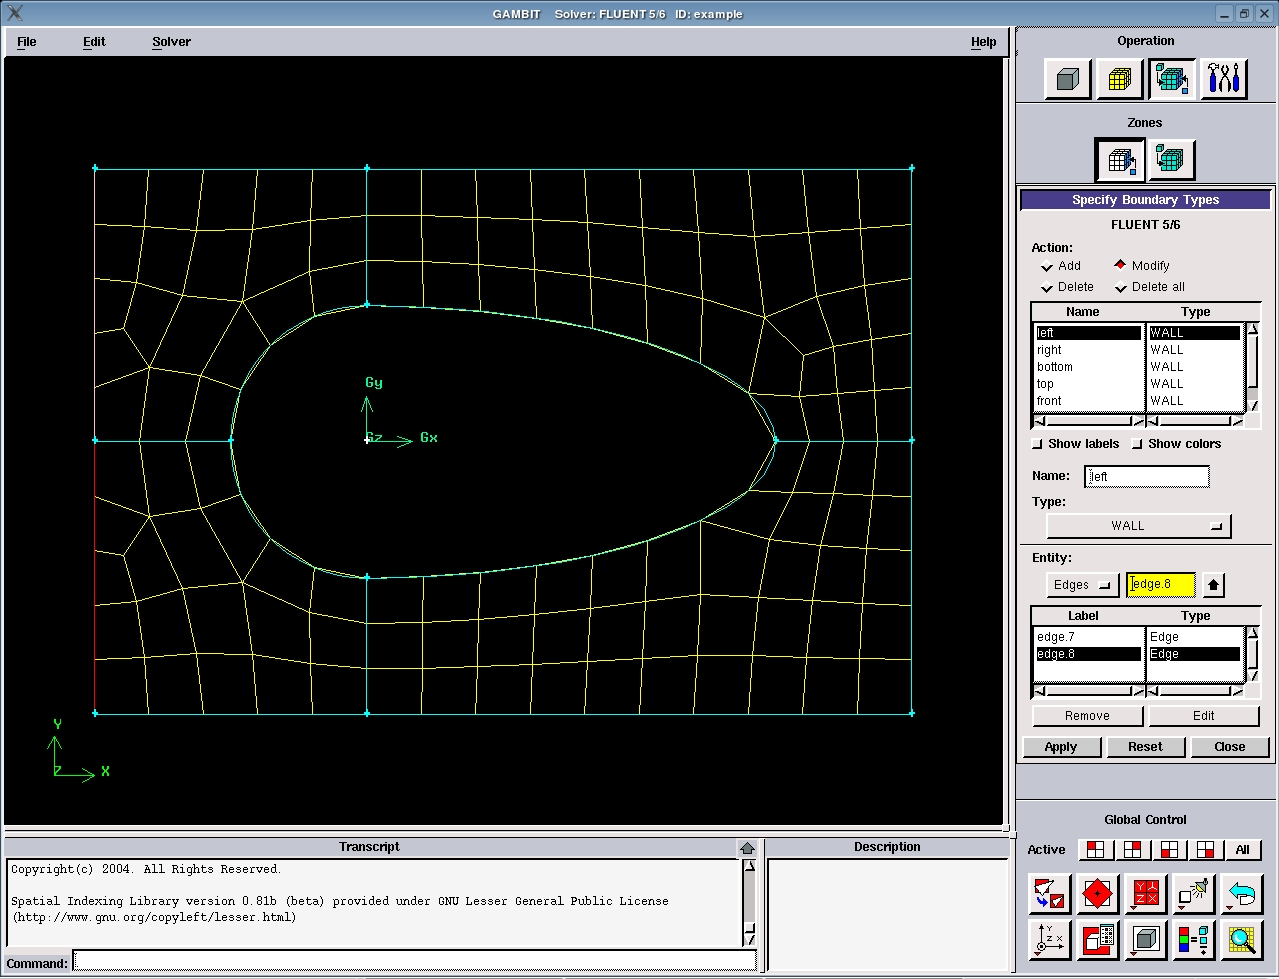
\includegraphics[scale = 0.26]{example01.jpg}
\caption{Den R"andern Namen geben und als WALL kennzeichnen}
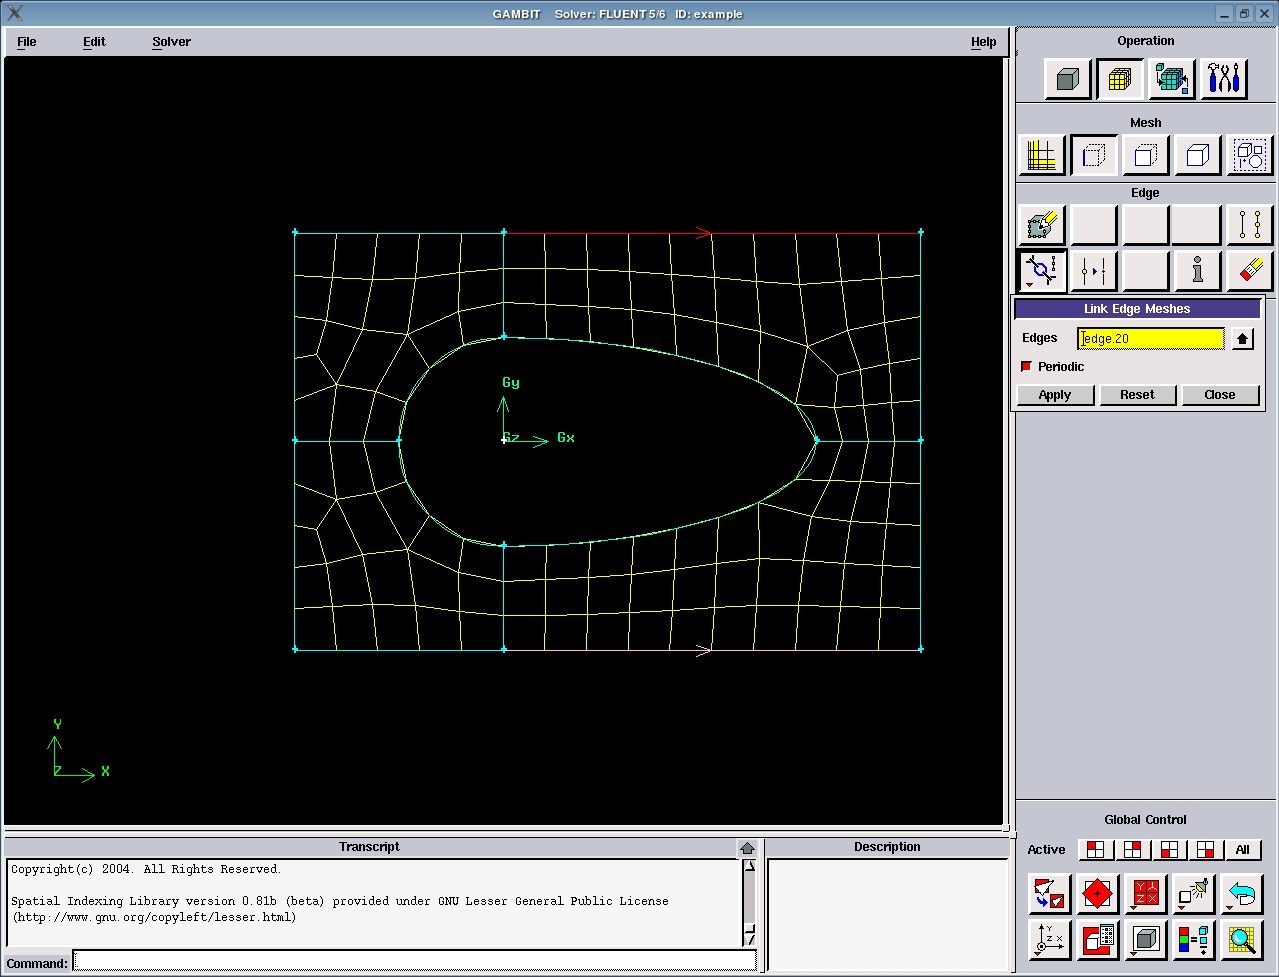
\includegraphics[scale = 0.26]{example03.jpg}
\caption{Periodische R"ander immer "`gekoppelt"´ vernetzen}
\end{figure}

Au"serdem ist es noch wichtig unter \verb|Zones| \(\to\) \verb|Specify| \verb|continuum| \verb|types| f"ur das gesamte vernetzte Gebiet (also alle dazu geh"orenden "`faces"´) ein Kontinuum vom Typ "`FLUID"´ zu erzeugen. Hier ist der gew"ahlte Name unwichtig.

Die fertige Gitterdatei wird im Hauptmen"u unter \verb|File| \(\to\) \verb|Export| \(\to\) \verb|Mesh| ausgegeben. Hier mu"s die Option \verb|Export| \verb|2-D| \verb|(X-Y)| \verb|mesh| markiert sein. Im vorliegenden Beispiel wird die Gitterdatei als "`example.msh"´ exportiert.

\newpage
\section{Aufbau der Input-Datei}

Um die fertige Gitterdatei (example.msh) in das Semtex-Format zu konvertieren ist au"serdem noch die Input-Datei (hier example.inp) notwendig. Sie enth"alt Information "uber die Randgeometrie und die sog. Rand-Gruppen (boundary groups).

Ganz am Anfang der Datei, unter dem Eintrag \verb|# case name for export| wird der Name der Semtex-Sessiondatei festgelegt (hier: \verb|casename| \verb|=| \verb|example|). Als n"achstes wird die mit Gambit erzeugte Gitterdatei unter \verb|# grid| \linebreak \verb|information| angegeben (hier: \verb|file = example.msh|). Die n"achsten zwei Eintr"age (\verb|xScale| \verb| = 1.000|, \verb|yScale| \verb| = 1.000|) erlauben es die Skalierung in x- oder y- Richtung zu ver"andern. Der Letzte Eintrag (\verb|type = 0|) gibt nur an, da"s die Gittertatei im FLUENT5/6 Format vorliegt. Der Converter kann vorl"aufig nur dieses Format interpretieren, deshalb braucht dieser Wert nie ver"andert zu werden. Danach kommen zwei gr"o"sere Abschnitte, die direkt mit der Behandlung der R"ander zu tun haben.

Zuerst wird f"ur jeden Rand im Abschnitt \verb|boundary curves| der Typ der Randgeometrie festgelegt.
Jeder Rand hat einen Namen, der ihm in Gambit zugewiesen wurde (z.B.: \verb|name = left|). Es wird festgelegt, ob der Rand aus Geradenabschnitten zwischen den Knotenpunkten (\verb|geom = 1|) besteht, oder ob die Randkurve mit kubischen Splines (\verb|geom = 4|) oder Kreisbogensegmenten (\verb|geom = 5|) beschrieben wird. 

\begin{description}
\item [Hinweis:] Die Werte \verb|geom = 2|, bzw. \verb|geom = 3| (jeweils f"ur Bernstein Approximation und B-Splines) werden nicht verwendet. Hier handelt es sich um "Uberbleibsel aus einer fr"uheren Version, die zwar im Quelltext des Converters noch vorhanden, in der aktuellen Version aber abgeschaltet sind.
\end{description}

Es gibt zwei verschiedene Varianten, wie kubische Splines verwendet werden k"onnen. Bei der ersten Variante werden die Elementknoten, die auf dem gekr"ummten Rand liegen, als Kontrollpunkte f"ur das Generieren einer Spline-Kurve verwendet. Die daraus erzeugte Kurve durchl"auft dann ganau alle diese Punkte. Sie wird in einer gesonderten Datei gespeichert, deren Namen sich aus dem "`casename"´ und dem Namen des jeweiligen Randes zusammensetzt. So hei"st die f"ur den Rand \verb|back| erzeugte Datei \verb|example_bndry-spline_back.dat|. Damit Semtex auf diese Datei zugreift, wird sie in der Eingabedatei unter dem Abschnitt \verb|<CURVES>| aufgef"uhrt.

Die zweite Variante ben"otigt eine vorher definierte Kurve als Ausgangsinformation. Diese Kurve mu"s als einfache Tabelle von x,y-Koordinaten in einer Textdatei gespeichert sein. Der Eintrag in der Input-Datei wird um die Angabe des Dateinamen erweitert, z.B.:

\begin{verbatim}
name = back, geom = 4, file='back_geometry.dat' /
\end{verbatim}

Nun wird der Converter diese Datei als Referenz benutzen und die Elementknoten auf dem gegebenen Rand so verschieben, da"s sie auf der Kurve liegen. In diesem Fall wird in der Semtex-Eingabedatei auf die urspr"ungliche Geometrie-Datei verwiesen und keine zus"atzliche Spline-Kurve generiert.

Wenn f"ur einen Rand Kreisbogensegmente verwendet werden sollen, ist es anstatt der Angabe einer Datei n"otig, die Koordinaten des Kreismittelpunktes festzulegen (z.B.: \verb|x0 = 0.0,| \verb| y0 = 0.0|).

\begin{verbatim}
name = front, geom = 5, x0 = 0.0, y0 = 0.0  /
\end{verbatim}

Der zweite gro"se Abschnitt befasst sich mit den Randbedingungen, bzw. mit den unter Semtex verwendeten "`boundary groups"´. Wieder gibt es f"ur jeden Rand einen Eintrag, zuerst kommt der Name, dann der zugeordnete "`key"´. Dieser key besteht aus nur einem Buchstaben. Er wird verwendet, um die R"ander in der Semtex-Sessiondatei den Randgruppen zuzuordnen, das hei"st, alle R"ander die z.B. ein "`w"´ als Key zugeordnet haben, stellen unter Semtex eine Randgruppe dar. In Semtex werden dann alle betroffenen Elementr"ander im Abschnitt \verb|<SURFACES>| mit diesem Key aufgef"uhrt.
Es ist m"oglich f"ur verschiedene R"ander denselben Key anzugeben. Da in der Semtex-Sessiondatei jedes Randelement einzeln mit dem zugeh"orgigen Key aufgef"uhrt wird, k"onnen verschiedene R"ander zu einer Semtex-Randgruppe geh"oren.
Prinzipiell sind alle Buchstaben als Key w"ahlbar. Einzige Ausnahme ist das \verb|p|, das zum kennzeichnen periodischer R"ander verwendet wird. Solche R"ander treten immer paarweise auf, und der zugeh"orige Rand mu"s angegeben werden 
(z.B.: \verb|name = bottom,| \verb|key = p,| \verb|link = top|, bzw. \verb|name = top,| \verb|key = p,| \verb|link = bottom|). Das Konvertierprogramm kann nicht erkennen, ob die Anzahl und Positionen der Knotenpunkte und die Abst"ande zwischen den Knoten auf den beiden R"andern "ubereinstimmen, deshalb mu"s dies schon in Gambit ber"ucksichtigt werden. Daf"ur gibt es beim Vernetzen der Beiden R"ander in Gambit die Funktion \verb|Link /| \verb|Unlink edges|, diese ist "uber das Toolpad zu erreichen.

\begin{figure}[hbp]
\centering
\verbatiminput{example.inp}
\caption{Inhalt der Datei \emph{example.inp}}
\end{figure}

\section{Erg"anzung der Semtex-Eingabedatei}

Damit die Eingabedatei mit Semtex verwendet werden kann, m"ussen noch einige Abschnitte hinzugef"ugt werden werden. Haupts"achlich die Abschnitte \verb|<FIELDS>|, \verb|<TOKENS>|, \verb|<GROUPS>| und \verb|<BCS>| sind f"ur die meisten Rechnungen mit Semtex notwendig. Mehr Information dazu kann der Dokumentation f"ur Semtex entnommen werden.

\end{document}